\section{Sistemas de diálogo}

Los sistemas de diálogo humano-computadora son cada vez más frecuentes, y sus aplicaciones comprenden una amplia gama de rubros: desde aplicaciones móviles, motores de búsqueda, juegos o tecnologías de asistencia para ancianos y discapacitados. Si bien es cierto que estos sistemas logran captar la dimensión lingüística de la comunicación humana, tienen un déficit importante a la hora de procesar y transmitir el aspecto superestructural de la comunicación oral, que radica en el intercambio de afecto, emociones, actitudes y otras intenciones de los participantes. Este problema puede verse en cualquier sistema que interactúe sintetizando lenguaje humano: por ejemplo, las aplicaciones telefónicas que atienden automáticamente a sus clientes \cite{pieraccini2005, raux2006}. Stanley Kubrick y Arthur C. Clarke predijeron esto a la perfección, cuando en ``2001: Una Odisea en el Espacio''(1968) dotaron a \emph{HAL} de una voz monótona y robótica, casi lobotomizada. Otro problema grave que sufren estos sistemas humano-computadora es que asumen que sus interacciones de ``a turnos'', cuando las conversaciones entre humanos suelen distar bastante de ese modelo.

Dentro de las cualidades del lenguaje oral, una de las más distintivas es la \emph{prosodia}, qué es la dimensión que capta \emph{cómo} se dicen las cosas, en contraposición a \emph{qué} se está manifestando. Posee varias componentes acústico-prosódicas: por ejemplo, el tono o pitch, la intensidad o volumen, la calidad de la voz, la velocidad del habla y otras. Un manejo adecuado de estas componentes es lo que, hoy día, distingue una voz humana de una artificial. Esta carencia de habilidad sobre la prosodia conlleva cierta dificultad en la interacción con agentes conversaciones, que suelen ser calificados como ``mecánicos'' o ``extraños'' en su forma de comunicarse. \cite{raux2006, ward2005}

En pos de mejorar el entendimiento entre agentes conversacionales y sus usuarios, resulta de vital importancia poder entender y modelar las variaciones prosódicas de la comunicación oral. Esto se traduciría tanto en una mejor apreciación de lo que quiere comunicar el usuario, como en una mayor naturalidad de la voz sintetizada por el agente.

\section{Mimetización}

En la literatura de Psicología del Comportamiento se ha observado con frecuencia que, bajo ciertas condiciones, cuando una persona mantiene una conversación, ésta modifica su manera de actuar aproximándola a la de su interlocutor. En una reseña de este tema se describe a este fenómeno como una ``imitación no consciente de posturas, maneras, expresiones faciales y otros comportamientos del compañero interaccional'' \cite[p. 893]{CHAR1999}  y conjeturan que es más fuerte en individuos con empatía disposicional. En otras palabras, personas con predisposición a buscar la aceptación social modifican su comportamiento en forma más marcada para aproximarlo a sus interlocutores

Esta modificación del comportamiento ha sido observada también en la manera de hablar. Por ejemplo, los interlocutores adoptan las mismas formas léxicas para referirse a las cosas, negociando tácitamente descripciones compartidas, en especial para cosas que resulten poco familiares \cite{BRE1996}. Estudios más recientes sugieren que esto también es cierto para el uso de estructuras sintácticas \cite{REI2006}. Este fenómeno subconsciente es conocido como mimetización, alineamiento, adaptación o convergencia y también con el término inglés \entrainment. Se ha mostrado que juega un rol importante en la coordinación de diálogos, facilitando tanto la producción como la comprensión del habla en los seres humanos\cite{nenkova2008, gravano2015backward}. En nuestro caso, nos interesa principalmente el \entrainment de la prosodia.

\section{Midiendo la mimetización}

Muchos estudios han examinado la mimetización prosódica, listados en \cite{DEL2013}. Un número importante de ellos se han basado en la premisa de la mimetización como un fenómeno lineal, en el cual la convergencia ``va sucediendo'' a lo largo de la conversación \cite{burgoon1995interpersonal}. Estos estudios dividen las conversaciones en varias partes, y verifican que la diferencia absoluta entre los valores medios (de las variables \ap) y sus desviaciones se aproxime en las últimas partes de la interacción. Sin embargo, este enfoque de la mimetización niega su faceta dinámica: los interlocutores pueden estar inactivos y luego hablar, pueden pasar por varias etapas como escuchar, pensar, discutir un punto, etc. En \cite{levitan2011measuring} se reportó que éste es un fenómeno no sólamente lineal, sino también dinámico, donde los interlocutores van coincidiendo en el análisis por turnos.

Un problema común que surge a la hora de calcular estas métricas es el hecho de que las conversaciones no están alineadas en el tiempo, ni se dan en turnos de duración constante. Nos preguntamos entonces qué partes del diálogo de un hablante deberían compararse con qué otras partes de su par. Un enfoque de comparar interlocuciones uno a uno es demasiado simple y no captura situaciones de diálogo reales, mucho más dinámicas y con solapamiento casi constante.

Teniendo en cuenta estos inconvenientes, utilizamos el método \TAMA(Time Aligned Moving Average) \cite{KOU2008}, que consiste en construir dos series de tiempo en base a cada interlocutor. Estas abstracciones son mucho más tratables que tener una secuencia de elocuciones de parte de cada hablante, y nos permiten efectuar análisis bien conocidos, uno de los cuáles nos permite construir una medida del \entrainment.


\section{Descripción TAMA}
\label{sec:ant_tama}

En \cite{KOU2008} se introdujo un método novedoso para el análisis del \entrainment acústico/prosódico. Esta técnica consiste, a grandes rasgos, en armar dos series de tiempo para cada uno de los interlocutores y luego utilizar herramientes de análisis sobre las series construídas. Una serie de tiempo, en términos coloquiales, es una colección cronológica de observaciones, como pueden ser los valores de las acciones de una empresa a lo largo del tiempo, o la cantidad de lluvia medida en \emph{ml} para cada mes de cierto año. En el apéndice \ref{sec:time_series} describimos más en detalle los conceptos básicos sobre series de tiempo.

Un problema que resuelve esta técnica es el del alineamiento: si intentásemos comparar cada segmento del habla (utterance) con otros, ¿cómo los alineamos? Una posibilidad sería uno a uno, aunque ésto es muy simplista y poco representativo de la realidad. Al introducir el concepto de series de tiempo, podemos olvidarnos de los segmentos del habla y simplemente utilizar estas construcciones.

Para construir la serie de tiempo de cada interlocutor debemos, en primer lugar, dividir el diálogo en ventanas solapadas de igual tamaño. A la diferencia entre ventana y ventana llamaremos \emph{frame step}, y al tamaño de ventana \emph{frame length}. Consideraremos sólo los segmentos de habla que se encuentren dentro de cada ventana; aquellos segumentos que atraviesen los límites de las ventanas son cortados para que se mantengan dentro de éste. En la figura \ref{tama} se ilustra el proceso.

Como producto de ésto, nuestro corpus queda dividido en una sucesión ventanas solapadas. En el trabajo original, se usa un step de 10 segundos, y un tamaño de ventana de 20 segundos. Ésto da como resultado un solapamiento del 50\%. En la sección \ref{sec:window_selection}, describimos la elección del tamaño de ventana que hicimos en base al corpus que utilizamos.

\begin{figure}
\centering
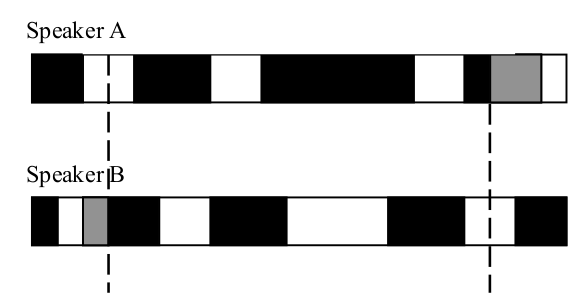
\includegraphics[width=10cm]{images/tama.png}
\caption{Gráfico de la separación del diálogo en ventanas}
\label{tama}
\end{figure}

Una vez que la conversación se ha partido en ventanas mediante el proceso descripto, se calculan los valores de la serie de tiempo para cada interlocutores de cada una de ellas. Ésto se hace mediante el siguiente cálculo:

\begin{equation}
    \mu = \sum\limits_{i=1}^N f_i d_i^\prime \label{eq:tama_mean}\\
\end{equation}

donde $i$ itera sobre las elocuciones dentro del \emph{frame}, $d_i^\prime$ es la duración relativa del segmento (respecto del tiempo total hablado) y $f_i$ es el valor de la \emph{feature} que estamos midiendo. $d_i^\prime$ se calcula con la fórmula

\begin{equation}
dr_i = \frac{d_i}{\sum\limits_{i=1}^N d_i}
\end{equation}

donde $d_i$ es la longitud en segundos de los segmentos del habla en el frame.

Como se ve en \ref{eq:tama_mean}, el valor que calculamos es una media ponderada del valor de la feature por la duración de las locuciones. Así, por ejemplo, al calcular una serie de tiempo sobre la intensidad, la contribución de interjecciones (\emph{ah!} por ejemplo), que suelen tener altos valores \emph{volumen}, estará disminuída por sus breves duraciones.

Una vez obtenidas, dado un feature acústico/prosódico y una conversación, dos series de tiempo mediante el cálculo ventana a ventana de \ref{eq:tama_mean}, necesitamos efectuar algún tipo de análisis sobre éstas para obtener una medida del \entrainment.

\nota{Mejorar el dibujo éste y agregarle una descripción}




\section{Objetivo del estudio}

En el presente estudio, aplicamos la técnica de \TAMA para definir dos métricas de \entrainment. Utilizamos un corpus de diálogo entre dos participantes angloparlantes, quienes interactúan mediante un juego a través de computadoras. El corpus ha sido anotado manualmente con variables que describen la percepción social de la conversación; por ejemplo: ¿el sujeto parece comprometido con el juego? ¿al sujeto no le agrada su compañero?

Luego, se analizará si existe, para cada una de las variables \ap,  alguna relación significante entre las métricas definidas y las percepciones sociales sobre las conversaciones. Uno esperaría que valores altos de nuestras métricas del \entrainment se relacionen con valores altos de variables sociales positivas, tales como mostrarse colaborativo o compenetrado en la tarea.
